\documentclass{article}
\usepackage{arxiv}

\usepackage[utf8]{inputenc}
\usepackage[english, russian]{babel}
\usepackage[T1]{fontenc}
\usepackage{url}
\usepackage{booktabs}
\usepackage{amsfonts}
\usepackage{nicefrac}
\usepackage{microtype}
\usepackage{lipsum}
\usepackage{graphicx}
\usepackage{float}
\usepackage{wrapfig}
\graphicspath{{../figures}}
\usepackage[square,numbers]{natbib}
\bibliographystyle{abbrvnat}
\usepackage{amsmath}

\usepackage{doi}


\title{Differential neural ensemble search with diversity control}

\author{K. Yakovlev, O.Bakhteev, K. Petrushina, P. Babkin
	%% David S.~Hippocampus\thanks{Use footnote for providing further
	%%	information about author (webpage, alternative
	%%	address)---\emph{not} for acknowledging funding agencies.} \\
	%%Department of Computer Science\\
	%%Cranberry-Lemon University\\
	%%Pittsburgh, PA 15213 \\
	%%\texttt{hippo@cs.cranberry-lemon.edu} \\
	%% examples of more authors
	%%\And
	%%Elias D.~Striatum \\
	%%Department of Electrical Engineering\\
	%%Mount-Sheikh University\\
	%%Santa Narimana, Levand \\
	%%\texttt{stariate@ee.mount-sheikh.edu} \\
	%% \AND
	%% Coauthor \\
	%% Affiliation \\
	%% Address \\
	%% \texttt{email} \\
	%% \And
	%% Coauthor \\
	%% Affiliation \\
	%% Address \\
	%% \texttt{email} \\
	%% \And
	%% Coauthor \\
	%% Affiliation \\
	%% Address \\
	%% \texttt{email} \\
}
\date{}

\renewcommand{\shorttitle}{differentiable ensembles search}

%%% Add PDF metadata to help others organize their library
%%% Once the PDF is generated, you can check the metadata with
%%% $ pdfinfo template.pdf
\hypersetup{
pdftitle={Differentiable algorithm for searching ensembles of deep learning models with diversity control},
pdfsubject={q-bio.NC, q-bio.QM},
pdfauthor={P.Babkin, K.Petrushina, K.Yakovlev, O.Bakhteev},
pdfkeywords={First keyword, Second keyword, More},
}

\begin{document}
\maketitle

\begin{abstract}
	
In our research we investigate a new method of sampling the deep learning models using
hypernetwork. A hypernetwork is a neural network which controls diversity of the models. It translates a real number into an architecture of a sampled neural network. This method samples deep learning models in one-shot regime, without any additional calculations losses.
To evaluate the performance of the proposed algorithm, we conduct experiments on the Fashion-MNIST and CIFAR-10
datasets and compare the resulting ensembles with ones sampled by other searching algorithms.

\end{abstract}


\keywords{ differential search \and neural ensembles \and hypernetwork \and diversity control }

\section{Introduction}

Nowadays methods of neural architecture search (NAS) are well-explored and proved to be an effective way of creating
more effective and efficient neural networks \citep{darts, robustify, xnas}. Some of these methods use different ways to smooth out the architecture so optimum for it can
be found by wide range of methods for smooth optimization problems. On the other hand, neural ensemble search (NES) is
modern and not as well investigated problem as NAS, although it is known that ensembles of deep learning models show better
results in different applied problems \citep{multi-head}.
Our paper investigates an method of sampling deep learning models in a new way that gives compatible results and has its own sphere
of implementations.

Our method takes the result of NAS as a base architecture than it samples architectures which are close to the optimal one in terms of Jensen-Shannon divergence (JSd). Architectures differ in terms of $\lambda$, idea of method is shown in \hyperref[fig:arch]{Fig. 1}. Basic architecture is gained with $\lambda = \lambda_1$.
Blue ellipses are equidistant surfaces of architectures. Staring with diverse parameter $\lambda = \lambda_2$ resulting architecture performs unacceptable accuracy, so architectures beyond the surface are not included into ensemble.
Method can control whether sampled architectures are close enough to the optimal one so they perform good accuracy on the original dataset and are diverse enough so every architecture makes its own contribution to the final answer.

\begin{figure}[h]
    \centering
    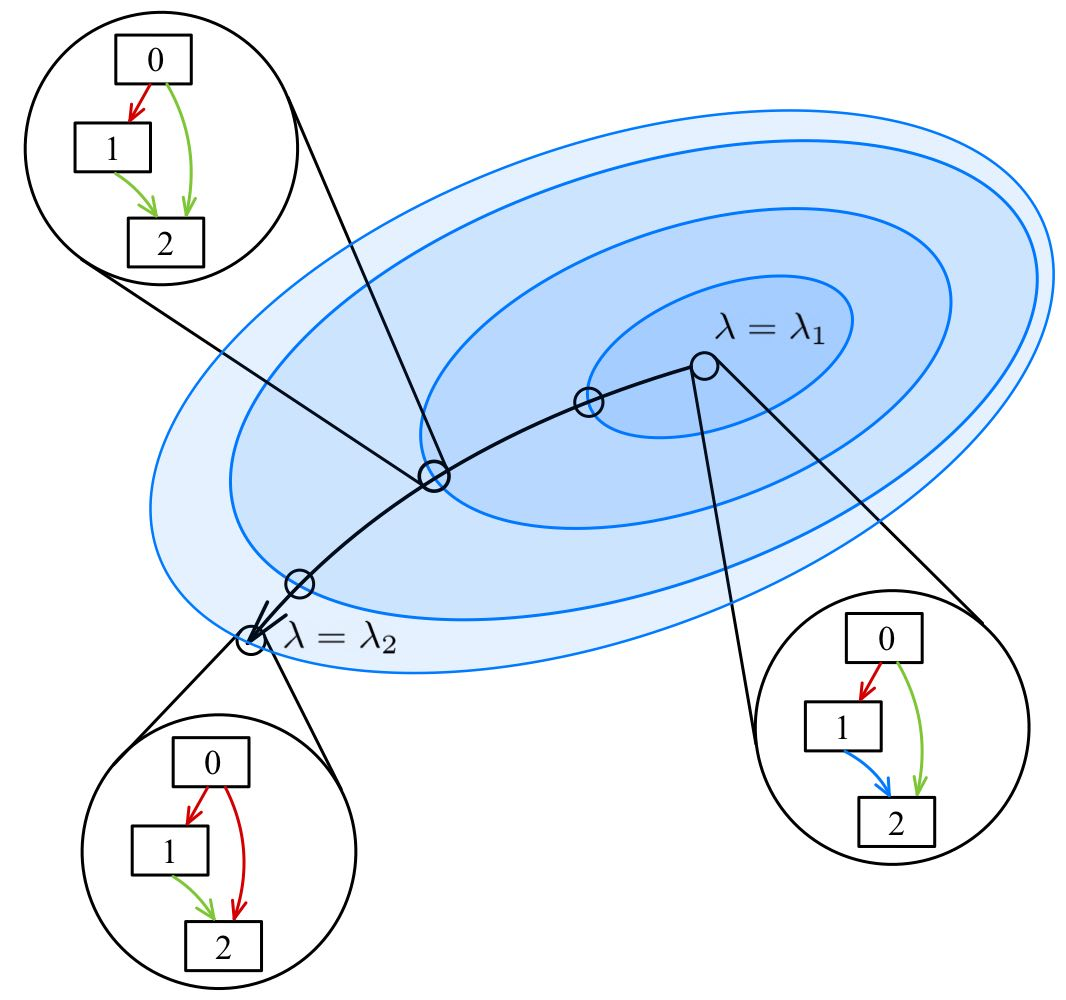
\includegraphics[width=0.6\textwidth]{fig1}
    \caption{\label{fig:arch}Architecture space}
\end{figure}

To sample architectures we use hypernetwork \citep{hypernetworks}. This network generates parameters for another network, which is called target network.
Previously hypernetwoks were intended to control different characteristics such as
complexity of architecture \citep{darts-cc} or parameters of the target model \citep{cont-learn} in several modern papers. In our paper it controls 
diversity of the target models, so every sampled model differs from previously sampled ones in terms of JSd.

The hypernetwork uses JSd to measure difference between two architectures which is symmetric and finite
in contrast to more popular Kullback–Leibler divergence. Our main idea of sampling different model is to use a regularizer,
based on JSd as a source of diversity.

This way we are able to sample deep learning models in one-shot, without and additional computational losses.
To sum up the scheme of our method: find a base architecture using DARTS, sample architectures in one-shot via differentiable algorithm. Inference answer is ensemble of the sampled deep learning models.

We conduct experiments on CIFAR and MNIST datasets to evaluate performance of the proposed method in terms of accuracy and time. Also we compare the performance with state-of-art NES and NAS algorithms \citep{darts, ???}.

\section{Problem statement}

Contrary to the selection of one single architecture in conventional NAS algorithm, this paper focuses on the problem of selecting a well-performing neural network ensemble with diverse architectures from the NAS search space, i.e., neural ensemble search (NES). In our formal statements
\mbox{\boldmath{$\alpha$}} denotes an architecture of a model, i.e. a set of operations between nodes. \mbox{\boldmath{$\alpha^*$}} is a NAS resulting architecture, i.e. an optimal architecture. \mbox{\boldmath{$w_\alpha^*$}} is vector of optimal parameters for architecture \mbox{\boldmath{$\alpha^*$}}. $\lambda$ is a measure of diversity, a real number from $0$ to $\Lambda$. \mbox{\boldmath{$\alpha$}}$(\lambda)$ is an architecture that corresponds $\lambda$, the architecture is gained after solving problem below. $f(\mbox{\boldmath{$w_\alpha$}}, \mbox{\boldmath{$\alpha$}})$ is an output of an architecture \mbox{\boldmath{$\alpha$}} and model parameter \mbox{\boldmath{$w_\alpha$}}. $S$ -- a set of architectures included into ensemble. $\mathcal{L}_{train}$, $\mathcal{L}_{val}$ are training and validation losses, respectively. We imply their dependence on preset dataset and do not denote it explicitly, because we do not deal with it.

Given the ensemble scheme, NES can be formally framed as

\begin{gather*}
	\min_S \mathcal{L}_{val}\left(\frac{1}{|S|}\sum_{\mbox{\boldmath{$\alpha$}} \in S}f(\mbox{\boldmath{$w_\alpha^*$}}, \mbox{\boldmath{$\alpha$}})\right) \\
s.t. \text{ }\forall \mbox{\boldmath{$\alpha$}} \in S \text{ } \mbox{\boldmath{$w_\alpha^*$}} = \arg \min_{\mbox{\boldmath{$w$}}} \mathcal{L}_{train}(f(\mbox{\boldmath{$w_\alpha^*$}}, \mbox{\boldmath{$\alpha$}}))
\end{gather*}

We rearrange the problem:  general for all architectures. Also architectures differ in terms of $\lambda$ so resulting functions can be calculated in terms of expected values.

\begin{gather*}
    \min_{\mbox{\boldmath{$\alpha$}}} \mathbb{E}_\lambda [\mathcal{L}_{val}(\mbox{\boldmath{$w^*$}}, \mbox{\boldmath{$\alpha$}}(\lambda)) - \lambda JS(\mbox{\boldmath{$\alpha^*$}}, \mbox{\boldmath{$\alpha$}}(\lambda))] \\
    s.t. \text{ } \mbox{\boldmath{$w^*$}} = \arg \min_{\mbox{\boldmath{$w$}}} \mathbb{E}_\lambda[\mathcal{L}_{train}(\mbox{\boldmath{$w$}}, \mbox{\boldmath{$\alpha$}}(\lambda))]
\end{gather*}

\subsection{Computational experiment}

In our model $\lambda$ is a random value, distributed according to uniform distribution from 0 to $\Lambda$ ($\sim U(0, \Lambda)$). Main goal of basic experiment is to estimate $\Lambda$ and also to investigate dependence of resulting architecture's performance on $\lambda$.

\subsubsection{Experiment planning}

In our basic experiment we run the algorithm on fashionMNIST dataset for several different $\lambda$ and looked at resulting architecture and accuracy. Further we will use $\lambda$ distributed randomly, but in basic experiment it is fixed.

\subsubsection{Preliminary report}

Obtained results are depicted in the table below. Maximal accuracy of sampled architectures is written down. Also we recorded amount of matched operations between nodes i.e. number of edges between particular nodes that contain the same operation in obtained architecture and the basic one.

This results allow us to choose $\Lambda = 32$. However amount of matching edges does not really coincide with our expectations. Architectures almost do not intersect. It can be explained by the fact that the optimized function is not convex, so algorithm fall into different minimums, however we can get more matching edges by using negative $\lambda$. 

\begin{table}[h   ]
	\caption{preliminary results}
	\centering
	\begin{tabular}{lll}

		\midrule
		$\lambda$     & accuracy, \% & matched operations \\
		\midrule
        0 (optimum) & 91.24 & - \\ 
        1/2  & 91.24 &  4   \\
		2  & 91.26   &  3   \\
		32 & 89.21   &  2   \\
		64 & 87.09   &  1   \\
		\bottomrule
	\end{tabular}
	\label{tab:table}
\end{table}

\section{Method}

Below we briefly described our method for solving problem of classification with dataset $\mathcal{D} = (\mathbf{X}, \mathbf{y})$. For each object $\mathbf{x} \in \mathbf{X}$ there is a label $y \in \mathbf{y}$. We solve the problem via NES, sampling architectures according to novel methodology which is formally described below.

\subsection{architecture}

Let $\mathcal{V} = \{ 1, \ldots, N \}$ be a set of vertices, where N is a number of vertices, and $\mathcal{E} = \{ (i, j) \in V \times V \mid i < j \}$ a set of edges between them.
$\mathcal{O}$ is a set of operations to choose from. Usually it contains pooling, convolutions, etc.
For each edge there is an operation $o \in \mathcal{O}$ that transits information from one node to another.

NAS algorithms search for optimal architecture. 
As it was mentioned below, architecture of neural network is a set of operations between nodes. In NAS methods architecture is a vector constructed by following rules. For each edge $(i, j) \in \mathcal{E}$, \mbox{\boldmath{$\alpha^{(i, j)}$}} is a vector, which assigns impact of each operation.
\mbox{\boldmath{$\alpha$}} is a concatenation of all structural parameters vectors \mbox{\boldmath{$\alpha^{(i, j)}$}}.

\subsection{reguralizer}

Source of diversity in out method is a regularizer with diversity parameter $\lambda$. By subtracting it from a loss function we promote method for finding an architecture which differs from the optimal one.

We use Jensen-Shannon divergence to measure diversity of two architectures. NES algorithms give discrete architecture as a result of their work, i.e. initially optimal architecture \mbox{\boldmath{$\alpha_{init}^*$}} is discrete, so JSd cannot be calculated with \mbox{\boldmath{$\alpha_{init}^*$}} as an argument. We smooth the architecture using smooth parameter $\tau$ to solve this problem. 
$$
\mbox{\boldmath{$\alpha^*$}} = (1 - \tau)\mbox{\boldmath{$\alpha_{init}^*$}} + \tau \frac{1}{|\mathcal{O}|}
$$

Assuming $\tau$ close to one we obtain a smoothed architecture that contains the same information about architecture as a initial one, but we also can use it in JSd.

\subsection{diversity control}

In order to control diversity we employ the concept of hypernetwork. A hypernetwork is a parametric mapping from $[0, \Lambda]$ to the set of model structural parameters \citep{darts-cc}.
$$
\mbox{\boldmath{$\alpha$}} : [0, \Lambda], \mathbb{R}^u \to \mathbb{R}^s
$$
Where $\mathbb{R}^u$ is a hypernetwork parametric space and $\mathbb{R}^s$ is space of model structural parameters. In this terms \mbox{\boldmath{$\alpha$}} can be redefined using hypernetwork

$$
\mbox{\boldmath{$\alpha$}} = \mbox{\boldmath{$\alpha$}}(\lambda, \mbox{\boldmath{$a$}}) \text{ or } \mbox{\boldmath{$\alpha^{(i, j)}$}} = \mbox{\boldmath{$\alpha^{(i, j)}$}}(\lambda, \mbox{\boldmath{$a^{(i, j)}$}})
$$
In this paper each function $\mbox{\boldmath{$\alpha^{(i, j)}$}}$ is a piecewise linear function
$$
\mbox{\boldmath{$\alpha^{(i, j)}$}}(\lambda, \mbox{\boldmath{$a^{(i, j)}$}}) = \sum_{k=0}^{N-1} \left( \frac{\lambda - r_k}{r_{k + 1} - r_k} \mbox{\boldmath{$a_k^{(i, j)}$}} + \left(1 - \frac{\lambda - r_k}{r_{k + 1} - r_k}\right) \mbox{\boldmath{$a_{k + 1}^{(i, j)}$}} \right) I[\lambda \in [r_k, r_{k+1}]]
$$

In our method $\lambda$ is sampled from predefined distribution $p(\lambda) = U(0, \lambda)$ and new architecture is obtained from hypernetwork.




\bibliography{references}

\end{document}